% Options for packages loaded elsewhere
\PassOptionsToPackage{unicode}{hyperref}
\PassOptionsToPackage{hyphens}{url}
\PassOptionsToPackage{dvipsnames,svgnames,x11names}{xcolor}
%
\documentclass[
  12pt,
  letterpaper,
  DIV=11,
  numbers=noendperiod]{scrartcl}

\usepackage{amsmath,amssymb}
\usepackage{setspace}
\usepackage{iftex}
\ifPDFTeX
  \usepackage[T1]{fontenc}
  \usepackage[utf8]{inputenc}
  \usepackage{textcomp} % provide euro and other symbols
\else % if luatex or xetex
  \usepackage{unicode-math}
  \defaultfontfeatures{Scale=MatchLowercase}
  \defaultfontfeatures[\rmfamily]{Ligatures=TeX,Scale=1}
\fi
\usepackage{lmodern}
\ifPDFTeX\else  
    % xetex/luatex font selection
\fi
% Use upquote if available, for straight quotes in verbatim environments
\IfFileExists{upquote.sty}{\usepackage{upquote}}{}
\IfFileExists{microtype.sty}{% use microtype if available
  \usepackage[]{microtype}
  \UseMicrotypeSet[protrusion]{basicmath} % disable protrusion for tt fonts
}{}
\makeatletter
\@ifundefined{KOMAClassName}{% if non-KOMA class
  \IfFileExists{parskip.sty}{%
    \usepackage{parskip}
  }{% else
    \setlength{\parindent}{0pt}
    \setlength{\parskip}{6pt plus 2pt minus 1pt}}
}{% if KOMA class
  \KOMAoptions{parskip=half}}
\makeatother
\usepackage{xcolor}
\setlength{\emergencystretch}{3em} % prevent overfull lines
\setcounter{secnumdepth}{5}
% Make \paragraph and \subparagraph free-standing
\makeatletter
\ifx\paragraph\undefined\else
  \let\oldparagraph\paragraph
  \renewcommand{\paragraph}{
    \@ifstar
      \xxxParagraphStar
      \xxxParagraphNoStar
  }
  \newcommand{\xxxParagraphStar}[1]{\oldparagraph*{#1}\mbox{}}
  \newcommand{\xxxParagraphNoStar}[1]{\oldparagraph{#1}\mbox{}}
\fi
\ifx\subparagraph\undefined\else
  \let\oldsubparagraph\subparagraph
  \renewcommand{\subparagraph}{
    \@ifstar
      \xxxSubParagraphStar
      \xxxSubParagraphNoStar
  }
  \newcommand{\xxxSubParagraphStar}[1]{\oldsubparagraph*{#1}\mbox{}}
  \newcommand{\xxxSubParagraphNoStar}[1]{\oldsubparagraph{#1}\mbox{}}
\fi
\makeatother


\providecommand{\tightlist}{%
  \setlength{\itemsep}{0pt}\setlength{\parskip}{0pt}}\usepackage{longtable,booktabs,array}
\usepackage{calc} % for calculating minipage widths
% Correct order of tables after \paragraph or \subparagraph
\usepackage{etoolbox}
\makeatletter
\patchcmd\longtable{\par}{\if@noskipsec\mbox{}\fi\par}{}{}
\makeatother
% Allow footnotes in longtable head/foot
\IfFileExists{footnotehyper.sty}{\usepackage{footnotehyper}}{\usepackage{footnote}}
\makesavenoteenv{longtable}
\usepackage{graphicx}
\makeatletter
\def\maxwidth{\ifdim\Gin@nat@width>\linewidth\linewidth\else\Gin@nat@width\fi}
\def\maxheight{\ifdim\Gin@nat@height>\textheight\textheight\else\Gin@nat@height\fi}
\makeatother
% Scale images if necessary, so that they will not overflow the page
% margins by default, and it is still possible to overwrite the defaults
% using explicit options in \includegraphics[width, height, ...]{}
\setkeys{Gin}{width=\maxwidth,height=\maxheight,keepaspectratio}
% Set default figure placement to htbp
\makeatletter
\def\fps@figure{htbp}
\makeatother

\RequirePackage{natbib}
% Add all necessary packages here
\usepackage{amsmath,amssymb,epsfig,tabularx,wrapfig}
\usepackage{graphicx}
\usepackage{color,soul}
\usepackage{verbatim}
\usepackage{ifthen}
\usepackage{psfrag}
\usepackage{siunitx}
\usepackage{enumerate}
\usepackage{hyperref}
\usepackage{setspace}
\usepackage{natbib}
% Formatting
\setlength{\topmargin}{-.5 in}
\setlength{\textheight}{9. in}
\setlength{\oddsidemargin}{.1in}
\setlength{\evensidemargin}{-.35in}
\setlength{\textwidth}{6in}
\font\heada=cmbx10 scaled\magstep3
\font\headb=cmsl10 scaled\magstep1
\font\headc=cmr8
\pretolerance=10000
\raggedright
\setlength{\parindent}{2 em}

% Define new commands
\newcommand{\bm}{\mathbf}
\newcommand{\PR}{\mathrm{P}}
\newcommand{\R}{\mathbb{R}}


\newcommand{\todo}[1]{\payAttention{red}{TODO}{#1}}

% Identifying information
\newcommand{\myname}{Ben DeVries}
\newcommand{\myadvisor}{Andy Hoegh}
\newcommand{\wprojcoord}{Ian Laga}  % Current Writing Project Coordinator
\newcommand{\maintitle}{Tree Based Models Applied to Flying Fox Areal Data}
\newcommand{\mydate}{Date of completion here as Month Day, Year}

\KOMAoption{captions}{tableheading}
\makeatletter
\@ifpackageloaded{caption}{}{\usepackage{caption}}
\AtBeginDocument{%
\ifdefined\contentsname
  \renewcommand*\contentsname{Table of contents}
\else
  \newcommand\contentsname{Table of contents}
\fi
\ifdefined\listfigurename
  \renewcommand*\listfigurename{List of Figures}
\else
  \newcommand\listfigurename{List of Figures}
\fi
\ifdefined\listtablename
  \renewcommand*\listtablename{List of Tables}
\else
  \newcommand\listtablename{List of Tables}
\fi
\ifdefined\figurename
  \renewcommand*\figurename{Figure}
\else
  \newcommand\figurename{Figure}
\fi
\ifdefined\tablename
  \renewcommand*\tablename{Table}
\else
  \newcommand\tablename{Table}
\fi
}
\@ifpackageloaded{float}{}{\usepackage{float}}
\floatstyle{ruled}
\@ifundefined{c@chapter}{\newfloat{codelisting}{h}{lop}}{\newfloat{codelisting}{h}{lop}[chapter]}
\floatname{codelisting}{Listing}
\newcommand*\listoflistings{\listof{codelisting}{List of Listings}}
\makeatother
\makeatletter
\makeatother
\makeatletter
\@ifpackageloaded{caption}{}{\usepackage{caption}}
\@ifpackageloaded{subcaption}{}{\usepackage{subcaption}}
\makeatother

\ifLuaTeX
  \usepackage{selnolig}  % disable illegal ligatures
\fi
\usepackage[]{natbib}
\bibliographystyle{plainnat}
\usepackage{bookmark}

\IfFileExists{xurl.sty}{\usepackage{xurl}}{} % add URL line breaks if available
\urlstyle{same} % disable monospaced font for URLs
\hypersetup{
  colorlinks=true,
  linkcolor={blue},
  filecolor={Maroon},
  citecolor={Blue},
  urlcolor={Blue},
  pdfcreator={LaTeX via pandoc}}


\author{}
\date{}

\begin{document}

%%%%%%%%%%%%%%%%%%%%%%%%%%%%%%%%%%%%%%%%%%%%
% Title page
\begin{singlespace}

\begin{titlepage}
\null
\vspace{2.in}
% Enter title here
\begin{center}
{\LARGE\bfseries \maintitle} \vspace{.1in}

\vspace{.05in}
{\LARGE\bfseries $\;$} \\ [.5in]
{\Large  \myname \\
\vspace{0.5cm}
Department of Mathematical Sciences \\
Montana State University \\ [.5in]}
\mydate \\ [1.in]
A writing project submitted in partial fulfillment\\
of the requirements for the degree\\[.25in]
Master of Science in Statistics
\end{center}
\end{titlepage}

%%%%%%%%%%%%%%%%%%%%%%%%%%%%%%%%%%%%%%%%%%%%
% Signatures
\begin{titlepage}
\null
\vspace{2.in}
\begin{center}
{\bfseries\huge APPROVAL}\\[1.in]
of a writing project submitted by\\[.25in]
\myname \\[1.in]
\end{center}
\noindent
This writing project has been read by the writing project advisor and
has been found to be satisfactory regarding content, English usage,
format, citations, bibliographic style, and consistency, and is ready
for submission to the Statistics Faculty.

\vspace{.3in}
\begin{center}
\begin{tabular}{ll}
\rule{2.75in}{.03in} & \rule{2.75in}{.03in} \\
Date& \myadvisor \\
& Writing Project Advisor \\
\end{tabular}
\end{center}

\vspace{1cm}

\begin{center}
\begin{tabular}{ll}
\rule{2.75in}{.03in} & \rule{2.75in}{.03in} \\
Date& \wprojcoord \\
& Writing Projects Coordinator \\
\end{tabular}
\end{center}

\end{titlepage}
\end{singlespace}


%%%%%%%%%%%%%%%%%%%%%%%%%%%%%%%%%%%%%%%%%%%%
% Abstract
\vspace{2.in}
\begin{abstract}
\begin{doublespace}
This is my abstract. Note that I'm using line breaks without trailing white spaces in this .tex file to
make version control work better. The XXXX is an important problem for researchers and this writing
project was written to provide a solution to this important problem. It contains an exploration
of the history of the problem, motivating its importance, an exploration of an application to
illustrate its importance, development and/or discussion of statistical software to apply
the solutions to the problem, a simulation study to explore the performance of the methods,
and a conclusion. It also contains useful references and an appendix containing code used.
Or maybe it doesn't do all this - it depends on what you do for your project.
\end{doublespace}
\end{abstract}


\newpage


\renewcommand*\contentsname{Table of contents}
{
\hypersetup{linkcolor=}
\setcounter{tocdepth}{3}
\tableofcontents
}

\setstretch{2}
\newpage

\section{Introduction}\label{sec:intro}

Flying foxes are a fruit bat, with around 65 species native to parts of
Asia, Australia, and Africa. In this project, we examine a population of
grey headed, and black flying foxes surrounding Ballina, New South Wales
Australia. Our interest in flying foxes stems from the Hendra virus,
which is endemic to the four species of flying foxes in Australia. This
rare virus is zoonotic, meaning it can be transferred from animals to
humans. There is a fairly low chance of bats transmitting Hendra virus
directly to people. Humans who have been infected with Hendra virus have
come into contact with horses exposed to waste/bodily fluids from flying
foxes.

Spreading a disease through an intermediate host of another species is
referred to as a disease spillover. In \emph{Pathogen Spillover Driven
By Rapid Changes in Bat Ecology}, \cite{andy_art} identified loss of
flying fox habitat and climate as influential factors in Hendra virus
spillovers. Loss of habitat and climate both effect the availability of
food and water, leading bats to venture into farmland and contaminate
water/food supplies intended for horses. Understanding what factors
influence flying fox feeding locations is thus naturally important to
public health. For our analysis, we examine the feeding locations of the
previously mentioned flying fox population, assessing whether any
associations with land cover may be drawn.

Our data on flying fox feeding locations is sourced from (). Data was
collected using a Robin radar, perched upon a hill within Ballina. The
radar is able to track many objects at once, providing us with the
flight path, velocity, classification, and other details. Traditionally,
human observers have been used to record location information for bats.
Manual counting is obviously labor intensive, and potentially less
precise than radar; especially after considering both black and
grey-headed flying foxes are nocturnal. It's easy to imagine potential
challenges in counting clouds of bats at dark. Additionally, the Robin
radar observes a larger region than manual observation. Instead of
counts at discrete observation sites, the Robin radar provides points
over a continuous space.

When exploring associations, background information is always important.
\cite{queens_lc} examined the potential spatio-temporal relationship
between changes in land cover and flying fox roost sites in Queensland,
Australia. In Kolkata, India, \cite{indian_lc} analyzed types of trees
and urban structures that attracted flying foxes with ANOVA. Both of
these studies utilized highly detailed land cover data that involved
manual survey. They also focused on differences in similar types of land
cover, whereas our land cover classes are broader but less specific. Our
end goal is not to perfectly describe the effects of land cover, but
rather to see what types of land cover may be associated with flying fox
feeding locations. Focusing on exploration, we turn to tree based models
due to their inferential capabilities and modelling flexibility.

We begin with a brief review of supervised learning before discussing
Classification and Regression Trees (CART) \cite{cart} along with
several models inspired by CART. Next, our attention shifts to tools for
obtaining and preparing data for our analysis. In this project we use
Google Earth Engine to obtain our covariates, and access the response
from an archived PostgreSQL database. Finally, we apply Bayesian
Additive Regression Trees (BART) \cite{bart_paper} to analyze the
feeding locations of flying foxes.

\section{Background}\label{sec:background}

\subsection{Supervised Learning}\label{supervised-learning}

In traditional regression models we assume some sort of relationship
between the response, variables of interest, and controlling factors.
Exploratory data analysis, background information, and model
experimentation can bring light to potential relationships, but many
problems involve unobservable dynamics that are difficult or impossible
to capture via a parametric model. In some cases it is often necessary
to take a more algorithmic approach to modelling. Unfortunately, many
models in the algorithmic framework are referred to as black boxes,
indicating the inner workings of a fitted model are difficult or
impossible to explain in a meaningful way.

Whether we choose to focus on predictive or explanatory modelling comes
down to our end goal, and often there is some degree of balancing the
two. For example, let's think about a model to classify whether someone
has a disease. Obviously we care about the predictive capabilities. If
the model is less accurate than an informed guess, it's not particularly
useful. Focusing solely on prediction and ignoring explainability, we
might implement a support vector machine. The support vector machine
model would project patients measurements into a higher dimensional
space and construct a hyper plane that separates the features into two
groups, diseased/not diseased. Now if a doctor were to tell his patient,
``We projected your measurements into a high dimensional space and
unfortunately you fell on the wrong side of the hyperplane'', the
patient is almost certainly walking out.

Our doctor can soften the delivery; for example, they might adjust a
patient's data and use the trained support vector machine to see how
changes affect the predicted outcome. But patients are likely to ask how
these changes impact their disease status. Logistic regression is a
great example of an explainable model. Using the logistic regression
model, the doctor might tell his patient ``Looking at individuals
similar to yourself, we've found an extra 30 minutes of exercise is
associated with decreasing the odds of disease by a factor of X'' Our
doctor still has to interpret a mathematical formula; and odds may be
somewhat abstract to the patient, but there is a concise explanation.

Decision tree ensembles sit within the black box framework, but the
explainability of individual trees has lead to establishing variable
importance and interaction measures along with other useful tools for
inference. It is still very difficult to interpret the effects of
individual predictors in these models, as the hierarchical structure can
make marginal effects very misleading. Still, variable importance
measures combined with predictive accuracy make ensembles of trees a
great tool for exploratory analysis.

Working with ensembles of trees, the models are not explainable in a
meaningful way as a individual prediction may involve hundreds or
thousands of decisions. We forego explaining an ensemble's reasoning and
instead ask two questions: How accurate is the model? And which
variables were useful in the model? If our model can make good
predictions, then variables deemed important have some sort of
association with our response, even if it's indirect.

Prediction based modelling has led to the development of a variety of
algorithms that focus on fitting the data as opposed to explaining it.
These algorithms can be much more complex than linear models. \emph{The
Elements of Statistical Learning} \cite{esl} was a key source for
understanding algorithms and concepts in statistical learning. This text
demonstrates situation where classic statistical models fall short,
showing how complex models can solve intricate problems. Algorithms are
explained in rigorous detail, while still providing intuition to
implementations and capabilities.

Our background discussion begins with some notation and concepts in
supervised learning. We then discuss the algorithms for several models,
using simulation to demonstrate their use. In supervised learning
problems, the goal is to map a set of features to a target. When
discussing these components, we'll follow the notation used in \emph{The
Elements of Statistical Learning} \cite{esl}. \(X\) denotes a features
while \(Y\) and \(G\) denote the target for quantitative and categorical
responses respectively. If there are \(N\) observations of \(p\) inputs,
then \(\bm X\) is an \(N\times p\) matrix. The features for the \(i\)th
observation are \(\bm x_i\) while \(\bm x_j\) denotes the vector of all
observations for the \(j\)'th feature.

A common approach in supervised learning is to assume our features and
target are observation of random variables with joint distribution
\(\text{Pr}(Y,X)\). \(G\) would replace \(Y\) in a classification
problem and \(\bm X\) would replace \(X\) for multiple covariates.
Letting \(\mathcal{X,\ Y}\) denote the supports of \(X, Y\), we want to
find a function \(f:\mathcal{X}\rightarrow\mathcal{Y}\) that predicts
\(Y\) reasonably well. To do this, we define a loss function
\(L(Y,f(X))\) which penalizes the prediction error on a training set
\(\boldsymbol \tau=(\bm x_1,y_1),...,(\bm x_N,y_N)\).

Our choice of loss function determines the optimal solution to the
problem. The expected prediction error (EPE) is defined as
\(\mathbb{E}[L(Y,f(X))]\). Our overall goal is to approximate the
function \(f\) that minimizes the EPE. Using squared errors for loss
\((L_2)\), the EPE is minimized by choosing \(f\) such that
\(f(x)=\mathbb{E}[Y|X=x]\) (The Elements of Statistical Learning, pg. 18
\cite{esl}).

Now we need an algorithm to approximate \(f\) using
\(\boldsymbol \tau\). Choosing an appropriate algorithm will be heavily
influenced by the availability and distribution of data. With a
quantitative target, we might be able to assume an additive error
relationship between \(Y\) and \(\bm X\).

The additive error model is simply \(Y=f(\bm X)+\epsilon\) where
\(\mathbb{E}[\epsilon]=0\) and \(\bm X\perp\epsilon\). Here we are
assuming the process that generated \(Y\) can be approximated using
\(\bm X\) such that the error due to ignored features and other factors
has mean zero. For data that was generated under an additive error
model, a natural approach to approximate \(f\) is to use a linear
combination of basis functions. A set of functions \(\mathcal{B}\) form
a basis if for every function \(f:\mathcal{X}\rightarrow\mathcal{Y}\),
there exists a unique linear combination of elements of \(\mathcal{B}\)
that is equal to \(f\). The additive model is defined as
\(Y=\beta_0+\sum_{j=1}^pf_j(\bm x_j)+\epsilon\).

One limitation of an additive model is we assume no interactions between
features. There's no reason we can't add interactions or functions of
multiple covariates, but identifying these interactions is difficult. We
might be able to fit a model with select transformations of covariates
and every possible interaction, but this would almost certainly result
in overfitting. Assuming a generating model with any form of noise
implies even the optimal \(f\) will not predict every observation
perfectly. A model is overfit when trends are ignored to explain slight
irregularities in a sample. Discerning irregularities is highly
subjective. Any decision we make based on observed data may lead to
overfitting. To compare models predictive capability, we use data that
has been held out from training to obtain a sample of prediction errors.
With this sample, we can use some metric (usually based on our loss
function) for model validation.

There are a variety of methods to perform model validation, but the two
most common are hold out and K-fold cross validation. In hold out, some
portion of the data is held out for testing and the rest is used to fit
the model. If the model contains hyper parameters, we could split the
data into training, validation, and testing. Fitting models to the
training set, we can try various values for hyper parameters and compare
model performance for predictions on the validation set. After we
determine the optimal hyper parameter values, we refit the model on the
combined training and validation set before using the testing set to
assess the final fit. In some cases, additional tuning may be required
after combining training and validation as additional training data may
change the optimal values of hyperparameters. Using training/testing
splits is generally favored for computationally intensive problems with
observations to spare. The primary disadvantage to hold out validation
is we can't use as much data for training.

In K-fold cross validation, we get to train and test using all available
data by first splitting the data into \(k\) folds of size
\(\approx N/k\). One fold is held for testing and \(k-1\) are used for
training. This is then repeated until all folds have been tested. A
metric can be then used to select the model before fitting it to the
complete dataset. K-fold makes the most of the available data, but is
more computationally expensive. Additionally, K-fold does not assess the
final model fit as parameter estimates will change as the model is
refit. For models with low variance, representativeness of the available
data is really the only concern. If there is a lot of variation in
estimated parameters across folds, our cross validation becomes more of
an assessment of the theoretical as opposed to fit model. This can still
useful for model selection and refinement.

\subsection{Decision Trees}\label{decision-trees}

Decision trees are a type of hierarchical model where the the feature
space is partitioned into hyperrectangular regions, and a model is fit
for each region. For regression tasks, we typically use mean only
models. In this case the decision tree model is a step function. Unlike
our mean only models for linear regression, we do not make any
distributional assumptions. Without a distribution, we can't quantify
the uncertainty in our predictions. Additionally, the binary structure
of trees changes the interpretation of effects. Small changes in a
continuous feature \(x_{i,j}\) may not effect the associated prediction
\(\hat y_i\). The mathematical relationship defining a linear model is
highly informative, but rather rigid. Trees greatly outperform linear
models with more complex data. A hierarchical structure naturally
handles multicollinearity, and can help us find interactions between
covariates. Even though we don't believe \(\bm X\) is related to
\(\bm y\) by a step function, we can gain insight to the true
relationship by a step function approximation. An example of a tree
model is shown in Figure~\ref{fig-tree-examp}. Every decision after the
top root node is conditioned on the previous decisions, allowing us to
display the hierarchy graphically.

\begin{figure}[H]

\centering{

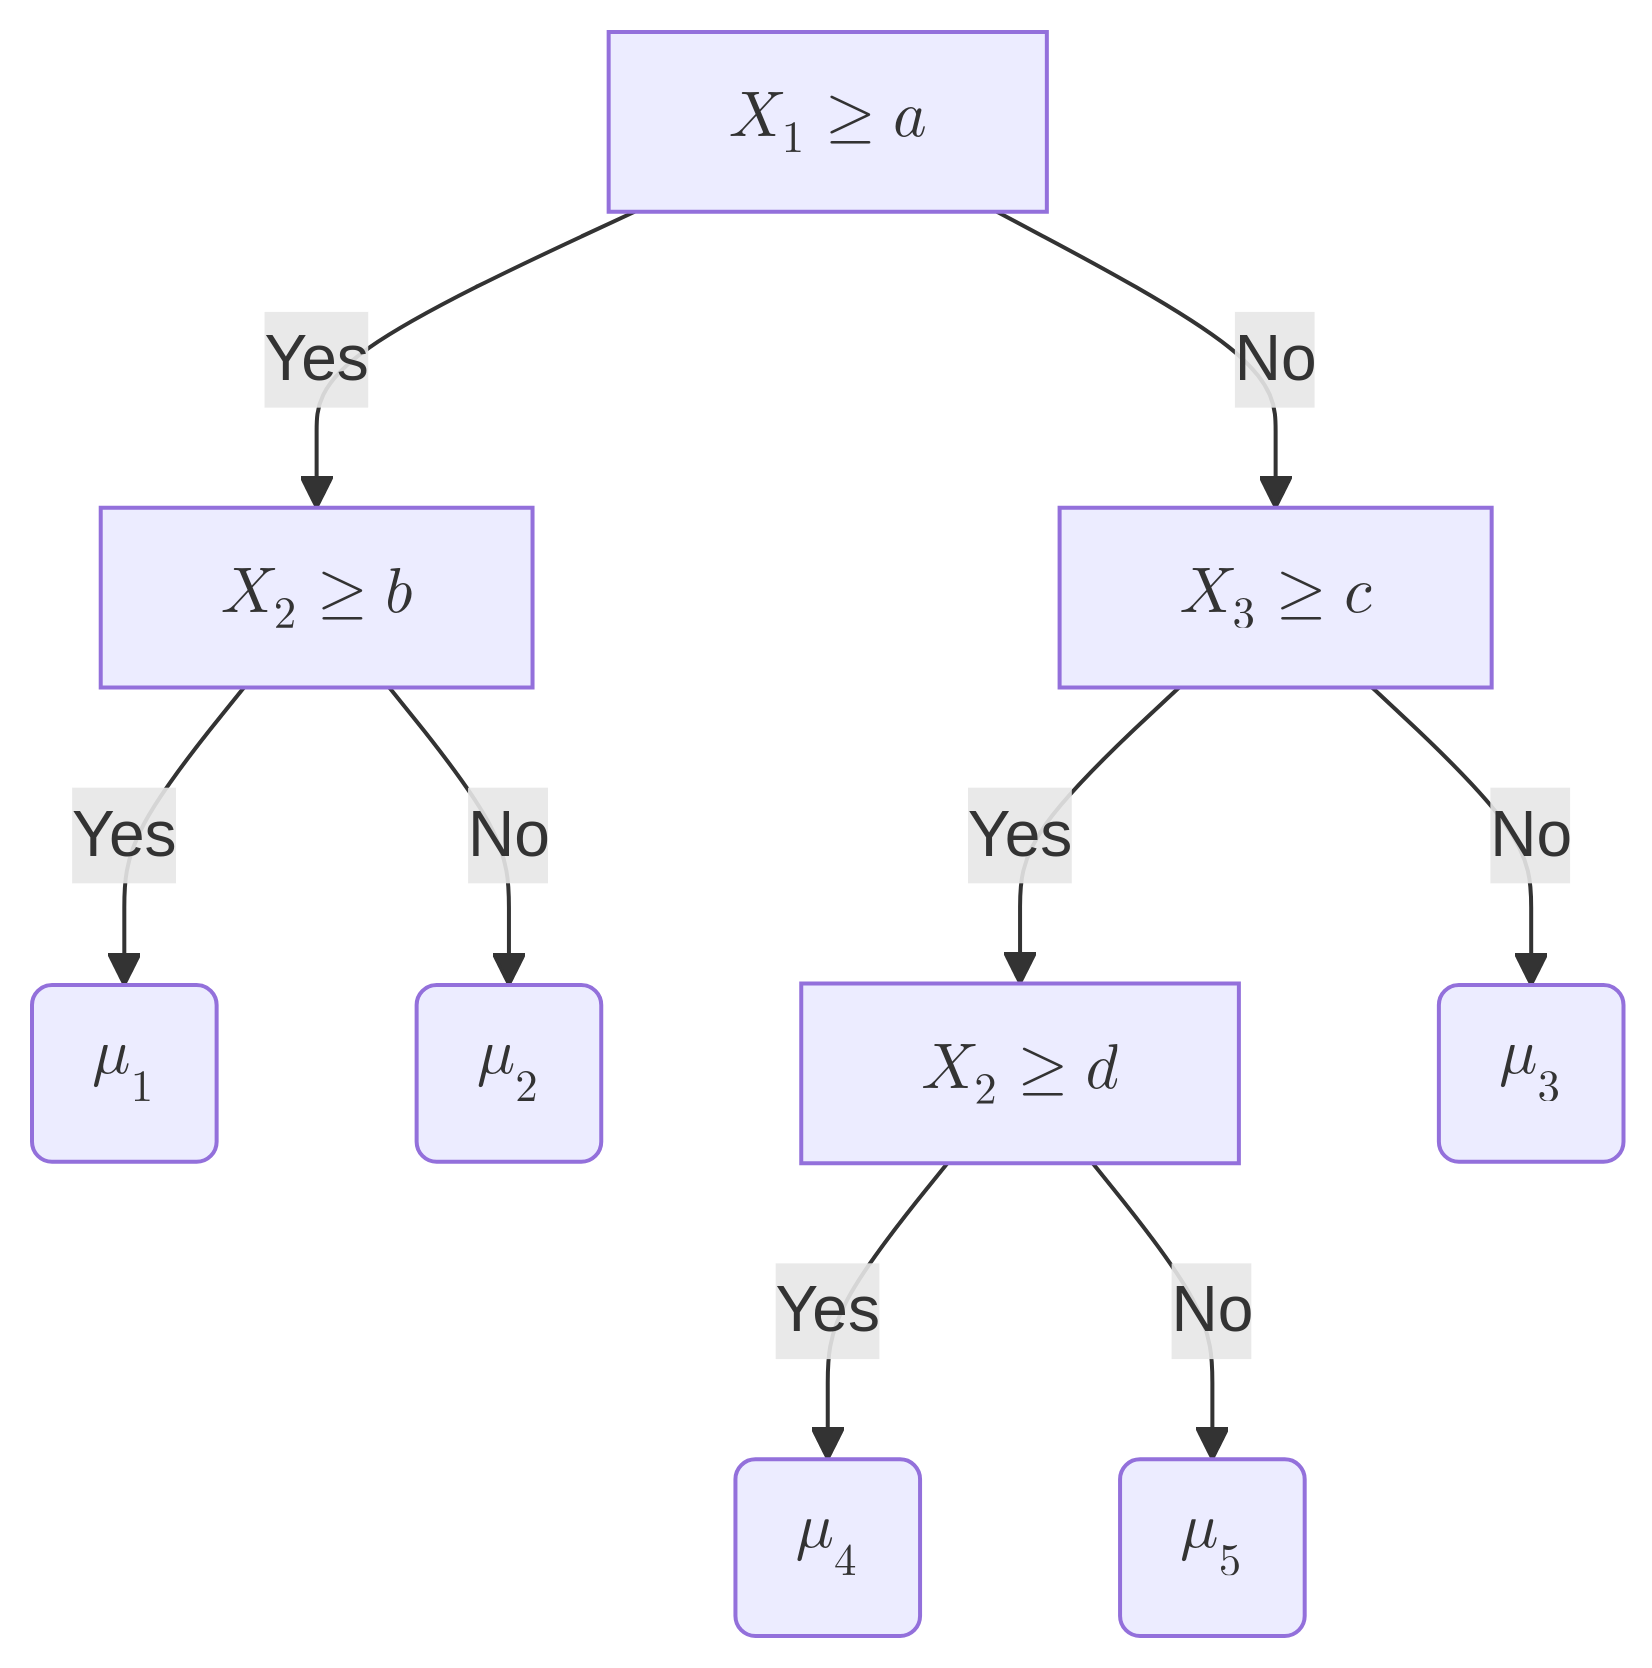
\includegraphics{figures/mermaid-figure-1.png}

}

\caption{\label{fig-tree-examp}Visualization of binary decision tree}

\end{figure}%

Step functions are very flexible. If there exists a function that can
map the features of our training data to the observed response, then we
can represent said function with a decision tree and achieve zero error
over \(\bm \tau\). With this flexibility, over fitting is a major
concern. We can control the overall size and shape of trees with three
hyper-parameters. First is the complexity parameter \(\alpha\).
\(\alpha\) scales the penalty which is based on the number of terminal
nodes (mean only models). Next we have the minimum split and minimum
bucket sizes. The minimum bucket is the fewest number of observations
allowed in a terminal node. Similarly, the minimum split is the least
number of observations allowed in one outcome of a binary decision. We
generally choose the complexity parameter by growing the largest
possible tree, then removing terminal nodes with fewer observations.
Next we compare the trees via cross validation and choose the tree with
minimal cross validated error. This process of choosing an appropriate
tree size is commonly referred to as pruning. While pruning helps reduce
the risk of over fitting, large regression trees are inherently
unstable.

When we say trees are unstable, we are essentially saying that a small
change to the data can result in a wildly different fit. We demonstrate
the variability in the structure of trees with a simulation study. Data
for the simulation study is generated under the model defined by
equations 1-4.

\begin{equation}\phantomsection\label{eq-a}{y_i=\cos(108t_i\sin(108t_i+w_i))\cdot\exp(\sin(108t_i\cos(108t_i+x_i)))+z_i}\end{equation}
\[W_i,X_i,Z_i\sim N(0,\sigma^2)\] \#eq-b\}
\begin{equation}\phantomsection\label{eq-c}{t_i=-\frac{\pi}{18},...,\frac{\pi}{18}}\end{equation}
\begin{equation}\phantomsection\label{eq-d}{i=1,2,...,350}\end{equation}

The rpart function developed by \cite{rpart} is used to fit our CART
model. A simulated testing data set displaying the true function along
with the fit from a tree chosen by cross validation on training is
displayed in Figure~\ref{fig-sim1-pred-vis}. Figure~\ref{fig-sim1-tree}
displays the number of splits for the optimal complexity parameter
chosen by cross validation.

\begin{figure}[H]

\centering{

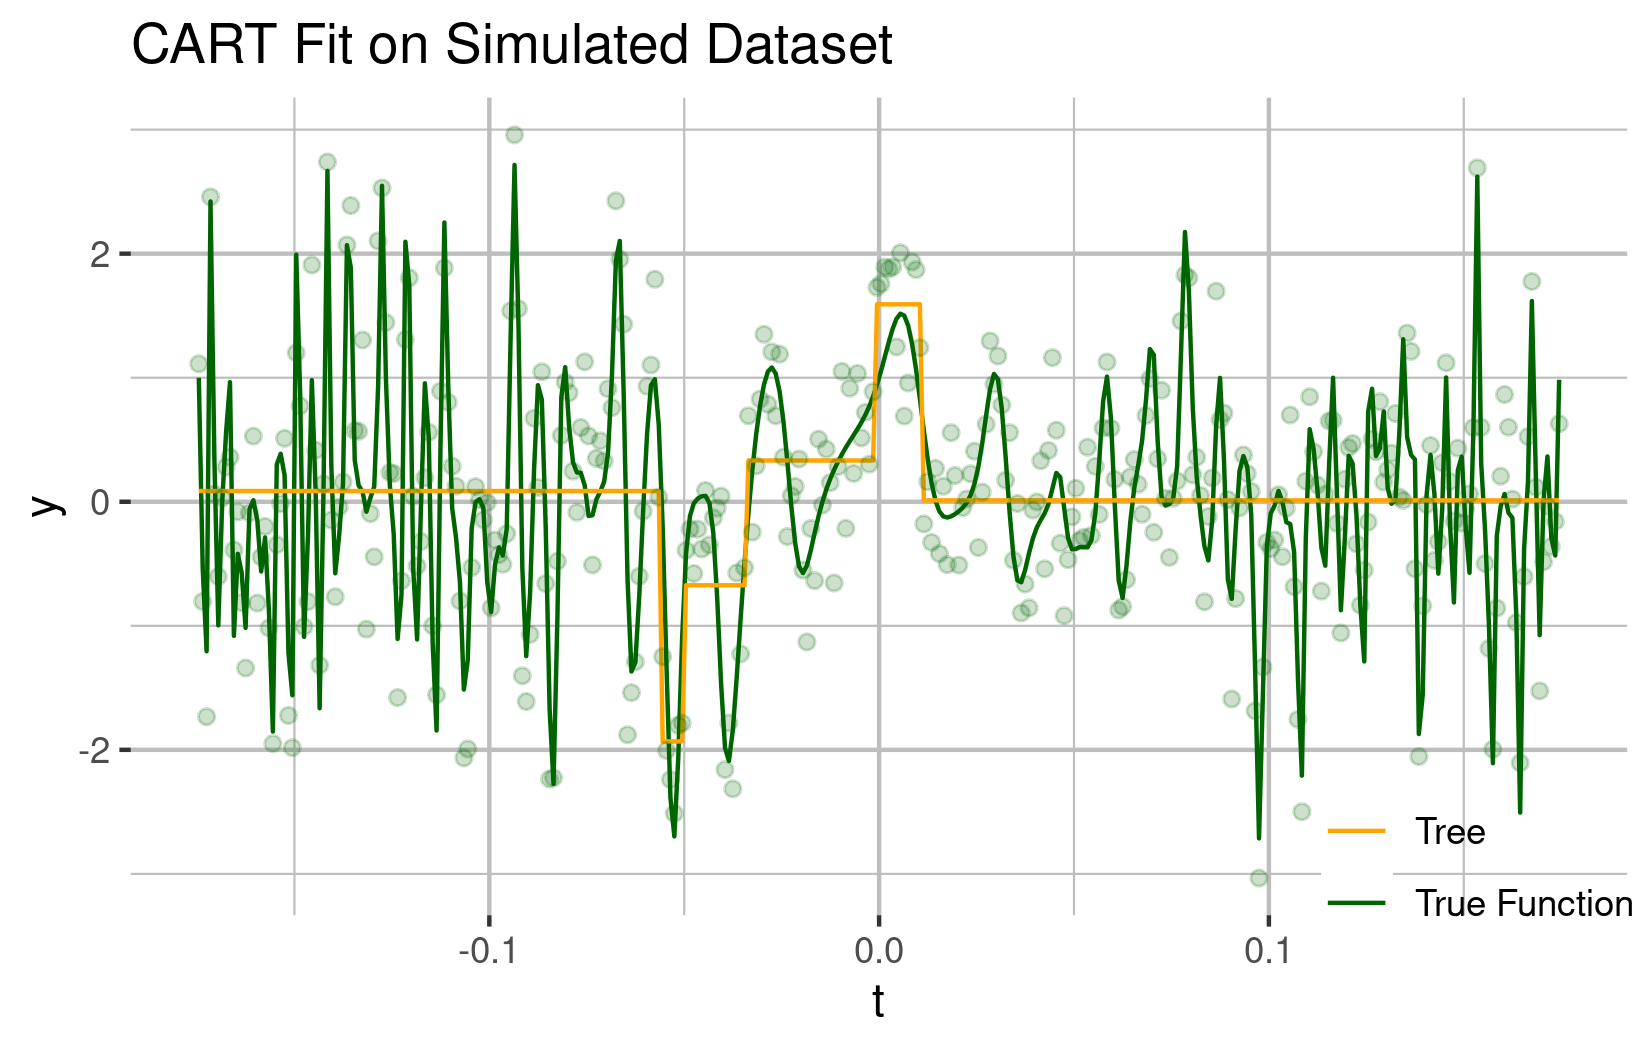
\includegraphics{main_QMD_files/figure-pdf/fig-sim1-pred-vis-1.png}

}

\caption{\label{fig-sim1-pred-vis}Visualization of simulated data and
predictions}

\end{figure}%

\begin{figure}[H]

\centering{

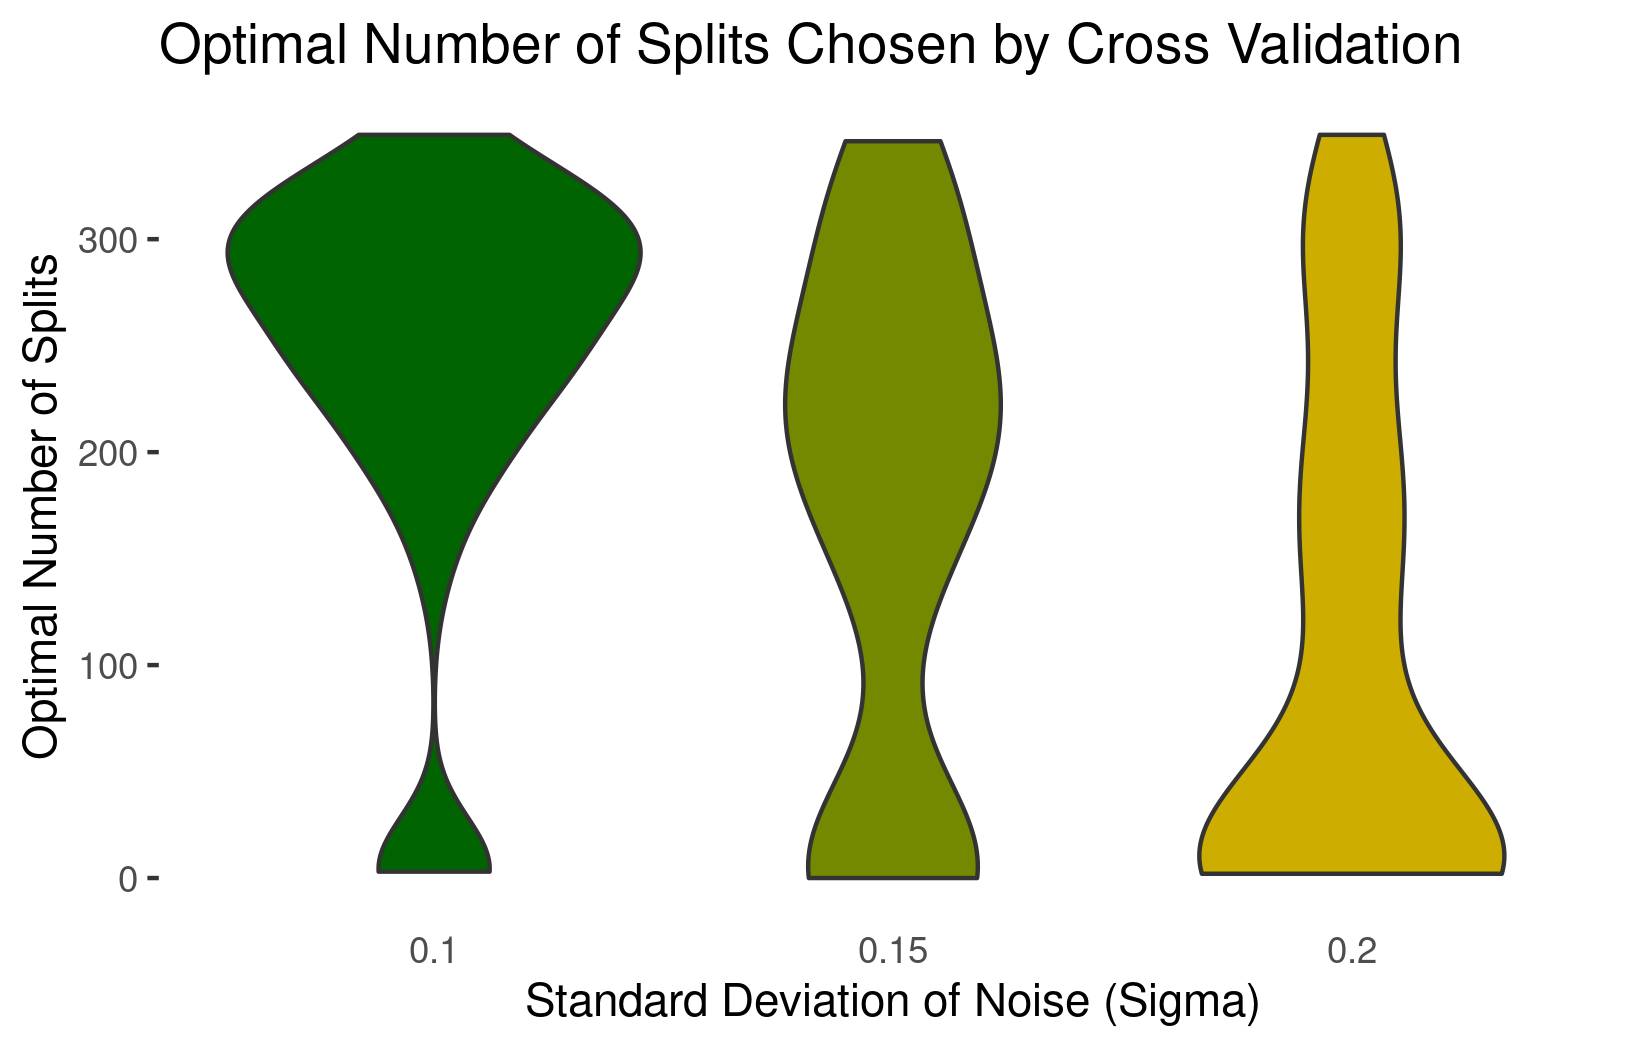
\includegraphics{main_QMD_files/figure-pdf/fig-sim1-tree-1.png}

}

\caption{\label{fig-sim1-tree}CART models can struggle with noisy data.}

\end{figure}%

Decision trees are very unstable for this data. Across all three noise
levels, the number of splits chosen by cross validation ranges from zero
to over 300. The variability in the size/structure of trees suggest we
can't have much faith in predictions from an individual tree. Slight
changes to the data could result in a completely different tree
structure, meaning our model may generalize poorly. A simpler model will
be less variable, but more biased. To maintain low bias and reduce
variance, we turn our attention to ensemble methods. Ensemble methods
are quite prevalent in predictive modelling. By combining the
predictions from several models, we can reduce the variance of
predictions while capturing complex intricacies of the data.

The random forests algorithm, developed by \cite{random_forest}, is a
CART-based ensemble combining Bootstrap Aggregating (Bagging)
\cite{bagging} and Ho's random decision forests \cite{Ho}. Bagging is
simply averaging the predictions of models fit to bootstrapped samples.
When possible, we obtain \(\hat y_i\) from averaging trees where
\(\bm x_i\) did not appear in training. These predictions are referred
to as ``out of bag predictions''. Cross validation on out of bag
predictions is not required as they are not based on the observed values
of \(\bm x_i\).

There's some intuition to the random forest algorithm. We know trees are
flexible, and bagging will allow models to consider variations in the
data. \emph{The Elements of Statistical Learning} present several proofs
demonstrating results that provide some intuition to the power of
bootstrapping. On pages 271-272, \cite{esl} show that the distribution
of bootstrap means for infinite samples from a normal population is
equivalent to to the Bayesian posterior distribution with a
non-informative prior. They also demonstrate that for the multinomial
likelihood, the bootstrap distribution with infinite draws from the
population approximates the Bayesian posterior assuming all outcomes are
equi probable apriori. Later on pages 282-288, \cite{esl} show that the
MSE of bagged estimates where samples are drawn from the population is
less than or equal to the MSE of an individual model. For classification
problems, \cite{bagging} shows that with infinite samples from the
population, bagging can approximate the optimal classifier under certain
conditions. This requires the majority of classifiers fit to
bootstrapped samples to predict the correct class more often than not
and relatively balanced classes. Otherwise, bagging can reduce accuracy.
All of these results concerning infinite samples are not very useful,
but hint at the practical applications of bagging.

The main limitation in bagging alone is correlation between models. When
averaging results from two trees \(T_1,T_2\), the variance of our
estimates will be
\(\frac{1}{4}(\mathbb{V}[T_1]+\mathbb{V}[T_2]+2\cdot\text{cov}(T_1, T_2))\).
If only a few variables contain relevant information, we expect trees to
make similar predictions. The random forests algorithm of
\cite{random_forest} combats the correlation between trees by taking the
same approach implemented by Ho in random decision forests, \citep{Ho}.
Random decision forests average multiple decision trees fit to the same
data. The key feature in the algorithm is the random subspace method
where a random subset of the available predictors is drawn for each
decision. Introducing randomness brings variety to the forest, resulting
in weaker correlation between trees. The combination of random subspace
and bagging makes Breiman's random forest a flexible model with low
variance. The hyperparameters for the random forest model are the number
of trees to grow, the minimum and maximum number of observations allowed
in a terminal node, and the number of predictors to select for each
decision. In Figure~\ref{fig-sim1-mse} we compare the MSE of models fit
to data simulated in the same way as the previous simulation study. The
rpart \citep{rpart} and randomForest \citep{rf_r} functions were used to
fit models.

\begin{figure}[H]

\centering{

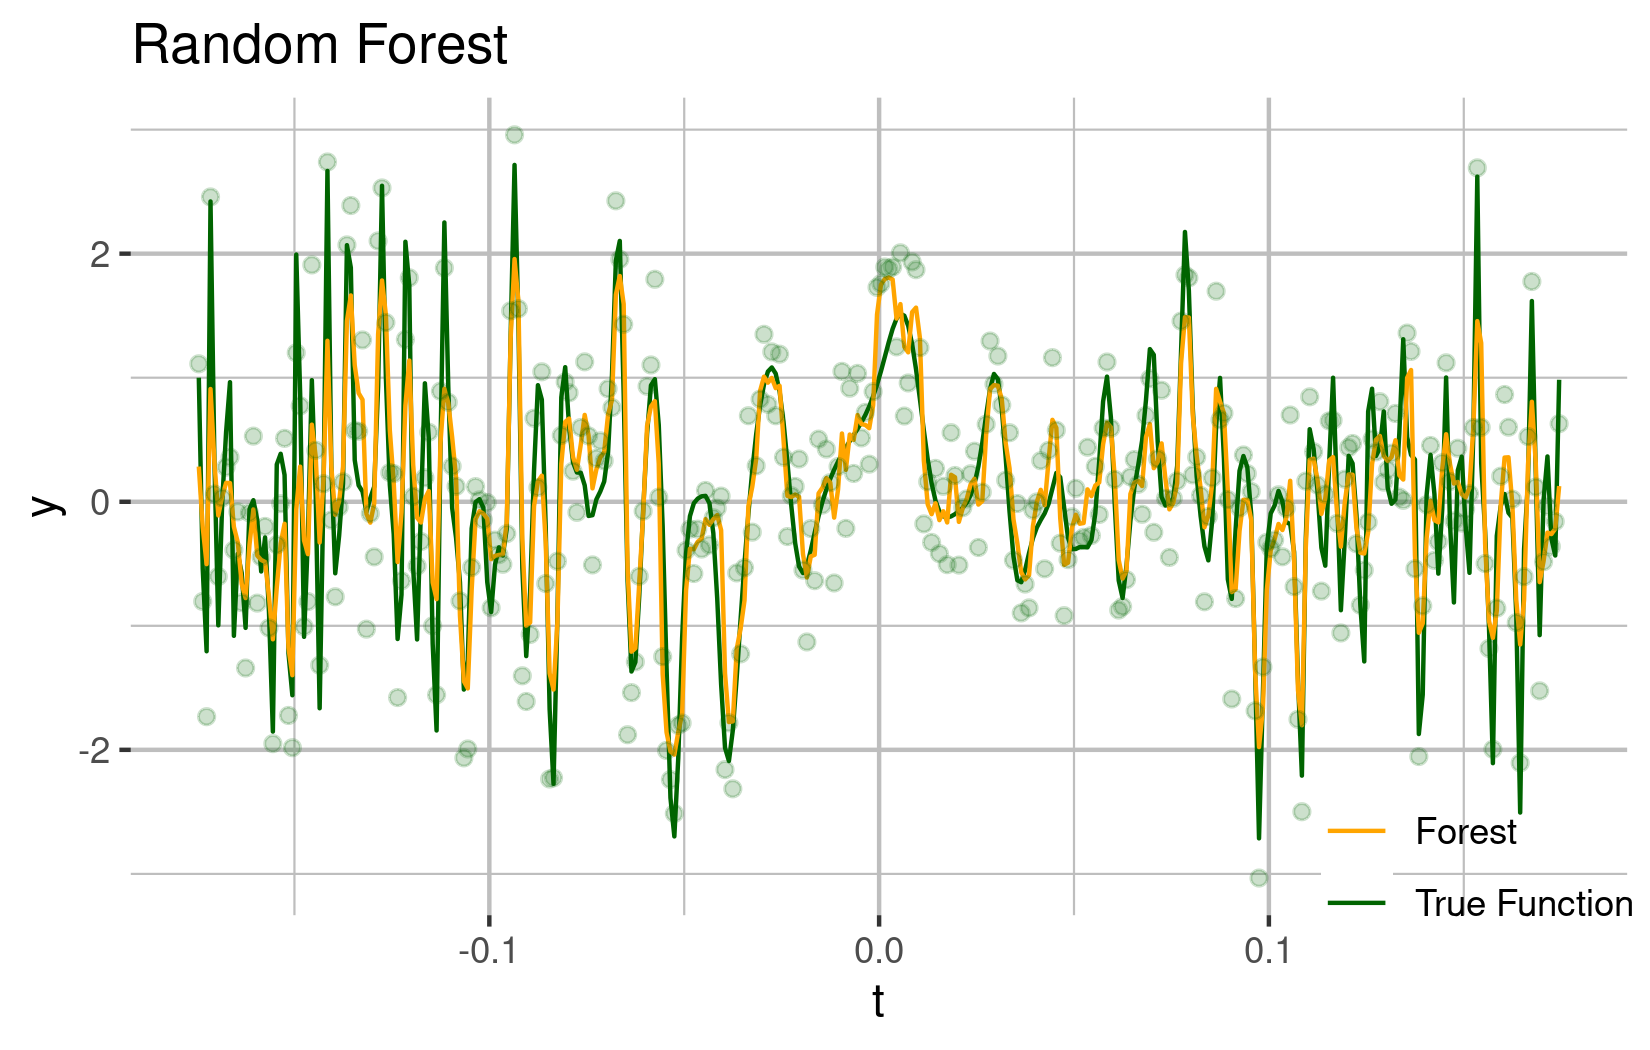
\includegraphics{main_QMD_files/figure-pdf/fig-sim1-rf-fit-1.png}

}

\caption{\label{fig-sim1-rf-fit}Violin plots of MSE for tree and forest
models on simulated data}

\end{figure}%

\begin{figure}[H]

\centering{

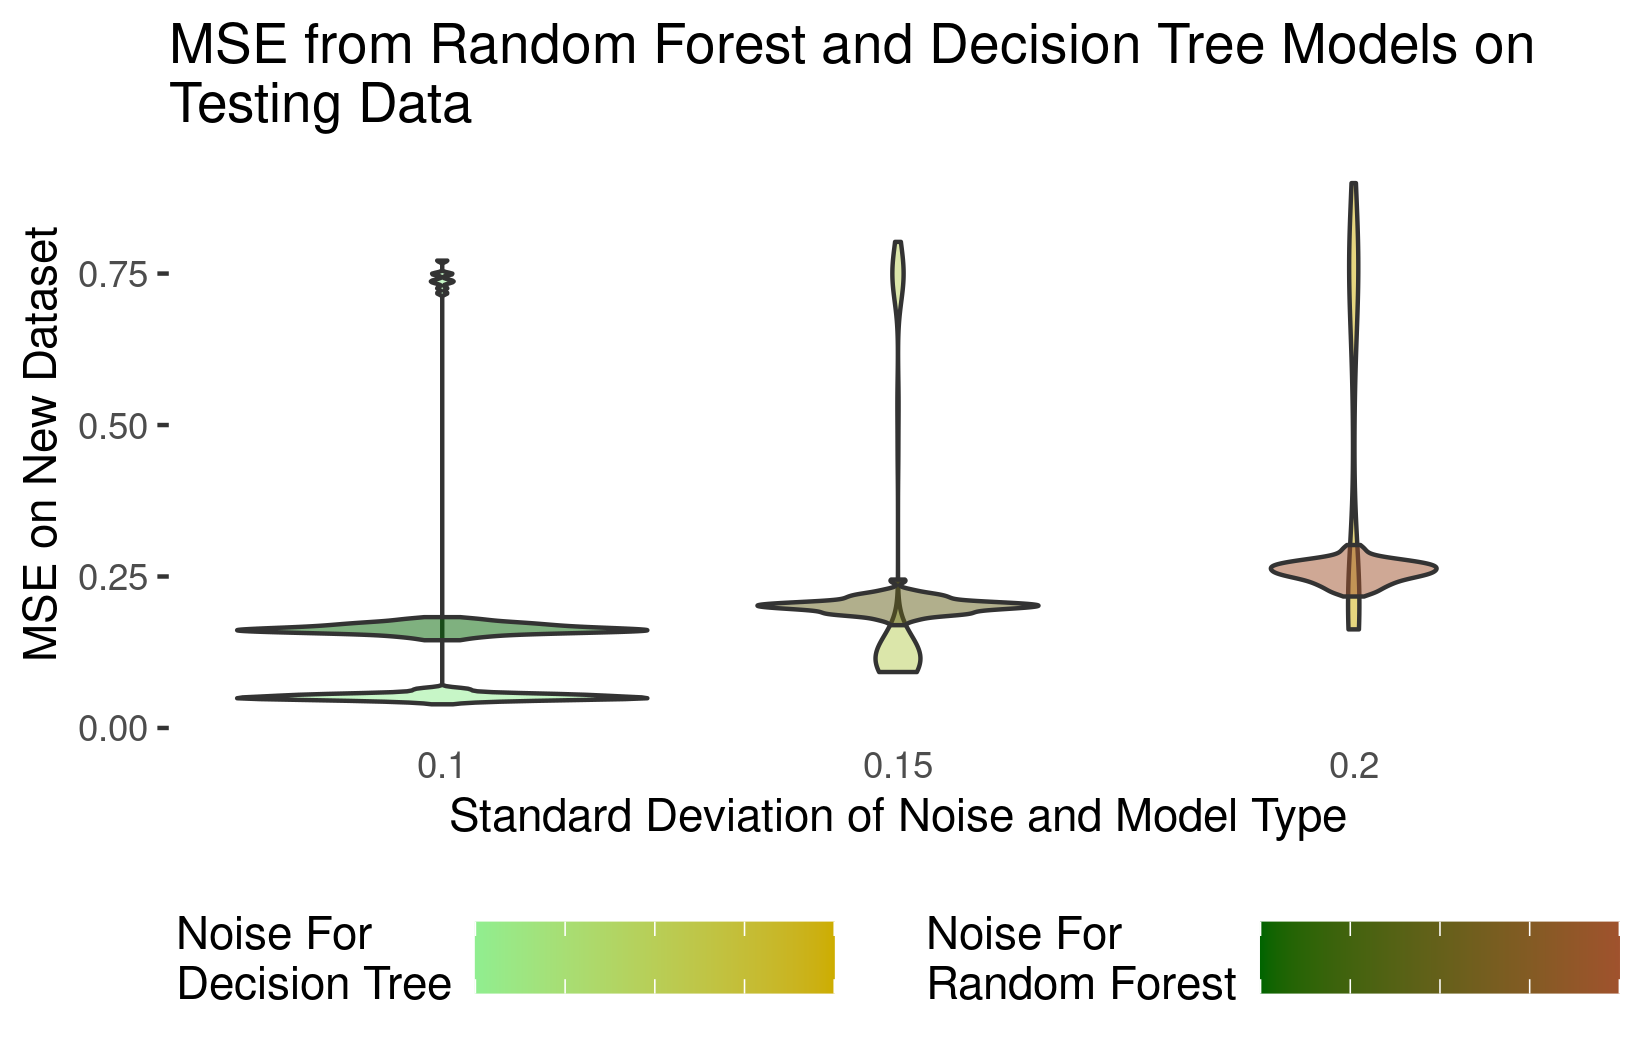
\includegraphics{main_QMD_files/figure-pdf/fig-sim1-mse-1.png}

}

\caption{\label{fig-sim1-mse}Violin plots of MSE for tree and forest
models on simulated data}

\end{figure}%

There is considerably less variation in the mean squared error of random
forests fit to the same data as individual decision trees, but single
tree models generally outperformed a random forest. Random forests are
designed for data with several covariates. With a single predictor, the
random forest algorithm degenerates to bagging with out of bag
predictions. Bagging reduces the variance of predictions at the cost of
bias, and thus the ``random forest'' predictions were often worse than
predictions from individual trees. Pages 600, 601 of The Elements of
Statistical Learning, \cite{esl} display a proof showing that the bias
of a random forest is the same as the bias of any individual tree in the
ensemble. The randomization in the random forest algorithm implies trees
within the ensemble are almost certainly smaller than a single tree fit
to the data. In cases where we have access to several predictors, large
trees will create complex hierarchies that are unlikely to exist in the
true model. The following simulation study shows the random forest
algorithm consistently outperform a single tree for data generated under
a linear model with correlated covariates. Violin plots of MSE on
testing data are displayed in Figure~\ref{fig-sim2}.

\begin{figure}[H]

\centering{

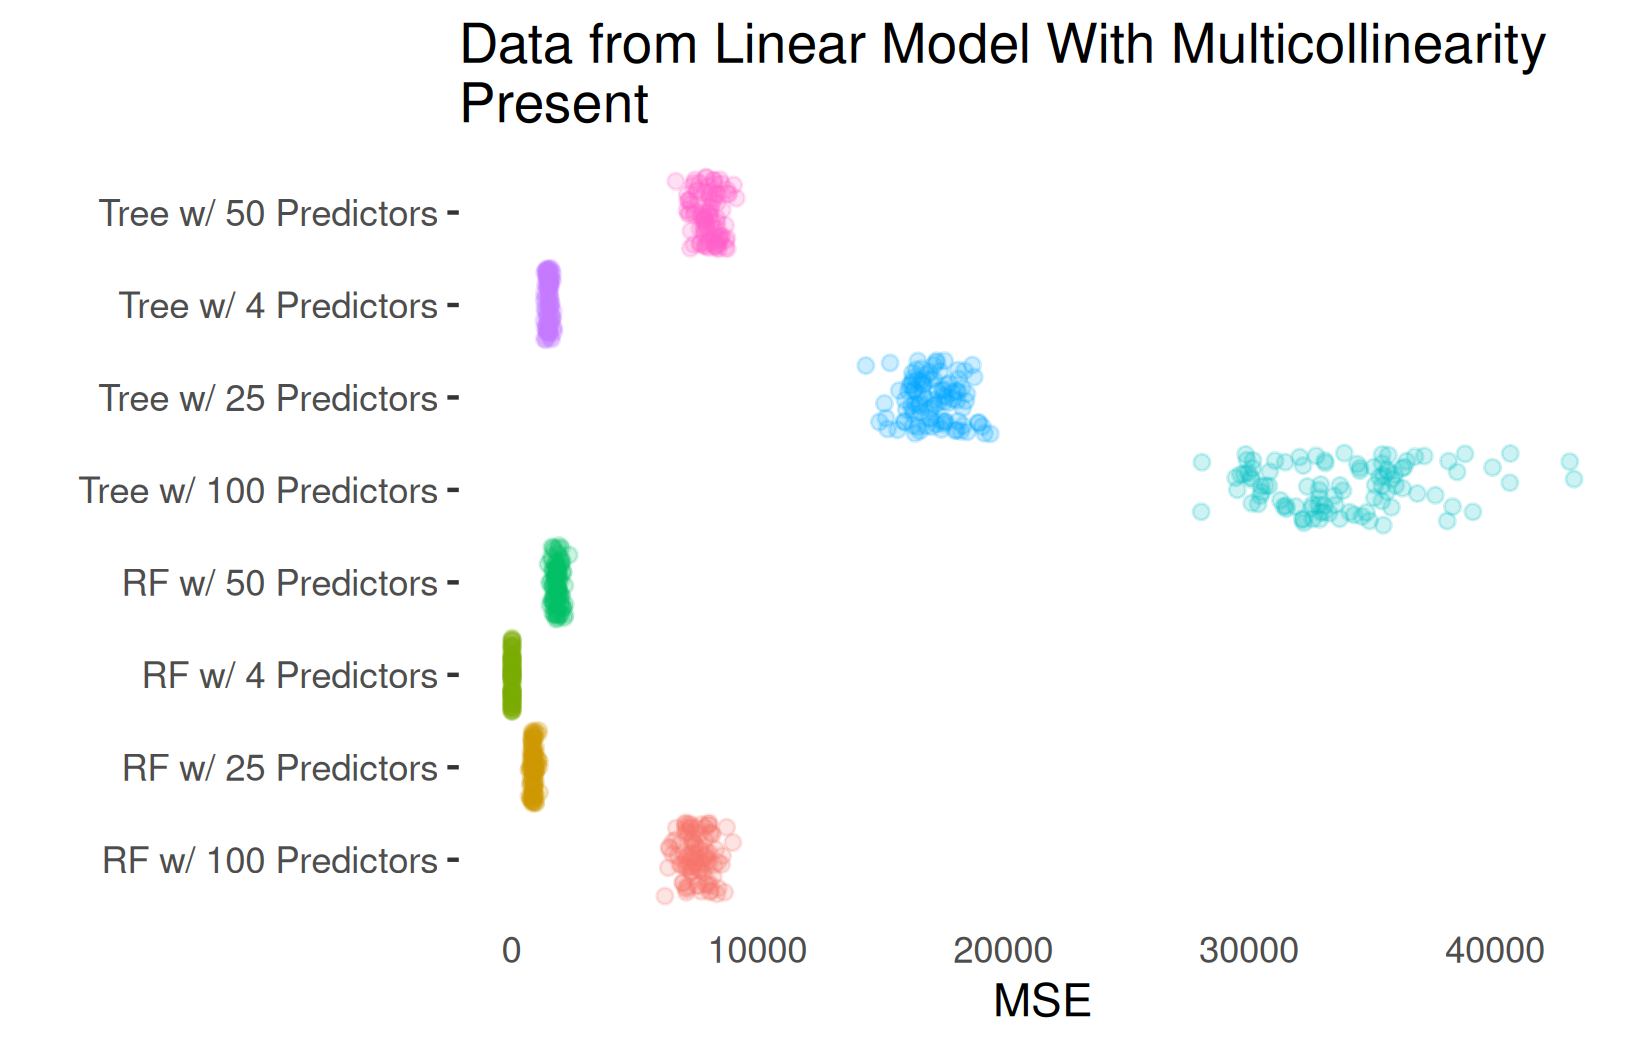
\includegraphics{main_QMD_files/figure-pdf/fig-sim2-1.png}

}

\caption{\label{fig-sim2}Violin plots of MSE for tree and forest models
on linear model with several predictors}

\end{figure}%

\subsection{Bayesian CART}\label{bayesian-cart}

Bayesian tree algorithms assume a stochastic process generates the tree,
and a distribution for the observations within the terminal nodes.
Randomness is used to explore possible structures that may increase the
posterior. The flexibility of trees necessitates regularization of their
structure, which can be easily achieved through the use of a prior.
There are many ways to specify a Bayesian tree but, our discussion is
limited to the Bayesian CART method proposed by \cite{bayes_cart}. In
Bayesian CART, the search process begins with an initial stump tree, and
proposes a new structure for the tree at random. For the proposal, there
are four possibilities. A change step is proposed with probability 0.4.
In the change step, a non-terminal node is randomly selected and the
splitting rule replaced. The new rule is chosen by randomly selecting a
splitting variable \(X_j\), and then randomly selecting an observed
value of \(\bm x_j\) as a cutoff. The same splitting rule cannot appear
multiple times within the current tree. For the grow step of the search,
a terminal node is randomly selected, a splitting rule is added, and a
sibling for the chosen node is grown. The probability a grow step is
0.25 and the decision rule is chosen in the same way as in the change
step. The third possible move in the search is randomly selecting
intermediate nodes, and collapsing all nodes beneath. This step is
referred to as pruning and is proposed with probability 0.25. The last
possible move for a trees structure is node swapping. Parent and child
intermediate nodes are selected and the rules are swapped. After
updating the structure of the tree, new nodes are marked as splittable
with probability \(\frac{\alpha}{1+\beta\gamma^d}\) where
\(\alpha\in(0,1)\) and \(\beta,\gamma\in(0,\infty)\) are hyperparameters
and \(d\) is the depth of the selected node. Finally, terminal nodes are
updated and the proposal is accepted or rejected. \cite{bayes_cart}
describe methods for independent and correlated terminal nodes. With the
proposal tree constructed, the Metropolis-Hastings algorithm is used to
update the sequence of trees.

Bayesian CART may become stuck around a local mode where the next tree
in the sequence provides little to no improvement. To combat this, a
sequence of trees is generated until the change in posterior probability
between trees in the sequence stabilizes. The algorithm is then
restarted to search for another local mode. Convergence is tracked by
comparing the posterior probability distribution of a tree to it's
predecessors, keeping track of which trees have the highest probability.
The frequency of tree structures explored is ignored, making Bayesian
CART a stochastic search as opposed to a Monte Carlo based method like
in BART. Averaging trees that have converged to a local mode results in
a model similar to random forests. Unlike random forests there is a
distribution for the predictions.

\subsection{Bayesian Additive Regression Trees
(BART)}\label{bayesian-additive-regression-trees-bart}

The other learning algorithm we explored was BART, or Bayesian Additive
Regression Trees. For a continuous predictor, BART assumes
\(y_i\sim N(\sum_{b=1}^m g(\bm x_i;T_b,M_b), \sigma^2)\) where \(T_b\)
is the \(b\)'th tree, \(M_b\) are the associated terminal nodes, and
\(g(\bm x_i;T_b,M_b)\) is the function that assigns \(\bm x_i\) to
\(\mu_{lb}\), \(l\in\{1,2,...,|M_b|\}\). Unlike the random forest
algorithm, the trees are not bagged and each tree has access to each
feature. Another key difference is the final model is based on the sum
of all trees as opposed to an average. BART models use the same
stochastic process to define the tree structure as Bayesian CART, but
differs in model specification. In Bayesian CART, trees that have high
posterior probability are recorded, but the number of occurrences for
each structure is ignored. This makes Bayesian CART a stochastic search
as opposed to a full MCMC. In BART, draws from terminal nodes remain
after the tree changes structure. We thus have a probability
distribution over the structure of the trees. Placing a highly
informative prior on the terminal status of nodes encourages smaller
trees, resulting in faster convergence and less variable predictions.

The algorithm starts by growing \(M\) trees with a single terminal node
(stumps). Gibbs sampling is used to alliteratively update each tree
conditioned on all other trees. Conditional updates are simplified by
expressing \(T_b|T_1,T_2,...T_{b-1},T_{b+1},...T_m\) as \(T_b|R_b\)
where \(R_b\) denotes the distribution of residuals from predictions
excluding \(T_b\). Summing trees grown conditionally on one another
makes the contributions of individual nodes small. \cite{bart_paper}
state ``\ldots{} we can imagine the algorithm as analogous to sculpting
a complex figure by adding and subtracting small dabs of clay.''
Conditional updates along with a highly informative prior on the
terminal status of nodes allow the model to explore intricate
relationships in the data, without overfitting.

BART is an adaptation of there original Bayesian CART algorithm
\cite{bayes_cart}. With the smaller tree sizes, the pruning proposal is
modified to only prune terminal nodes. Even with this modification,
trees will still collapse to a stump throughout MCMC. Convergence is
aided by the somewhat unrealistic assumption of independent priors for
each tree and the standard deviation. The joint prior is given by
\[p((T_1, M_1), (T_2, M_2),...,(T_m, M_m),\sigma^2)=p(\sigma^2)\prod_{b=1}^mp(M_b|T_b)p(T_b)\]
where \(p(M_b|T_b)=\prod_{l=1}^{|M_b|}p(\mu_{lb}|T_b)\), and
\(p(\sigma^2)\sim\nu\lambda/\chi^2_\nu\) with hyperparameters
\(\nu,\lambda\). The hyper parameters are selected by first choosing a
point estimate \(\hat\sigma\). By default, this is the residual standard
deviation for a multiple linear regression model. \(\nu\) is then fixed
(\(\nu\in[3,10]\) recommended) and \(\lambda\) solved for by imposing
the constraint \(\text{Pr}(\sigma<\hat\sigma)=q\), where \(q\) is an
additional hyper parameter. In the prior for a tree \(p(T_b)\), the
probability that a node at depth \(d\in\mathbb{N}\) is non-terminal is
given by \(\alpha(1+d)^{-\beta}\),
\(\alpha\in(0,1),\ \beta\in[0,\infty)\). A discrete uniform prior
imposes the initial belief that each feature equally likely to be
selected for a nodes splitting rule. Similarly, a discrete uniform
across the observed values of the selected predictor serves as the prior
for the cut point in the binary decision. A
\(N(|M|\mu_\mu,|M|\sigma^2_\mu)\) prior is assumed for each
\(\mu_{lb}|T_b\) where \(|M|\) is the total number of terminal nodes
across all trees. The hyperparameters \(\mu_\mu\) and \(\sigma_\mu\) are
chosen based on the data such that
\(\min(Y)=|M|\mu_\mu-k\sqrt{|M|}\sigma_\mu\) and
\(\max(Y)=|M|\mu_\mu-k\sqrt{|M|}\sigma_\mu\). In \cite{bart_paper}, they
recommend choosing \(k\in[1,3]\). The BART R package \cite{bart_r}
resales \(Y\) such that \(Y\in[-0.5, 0.5]\) and chooses
\(\mu_\mu=0\implies\sigma_\mu=\frac{0.5}{k\sqrt{|M|}}\).

Two differences between BART and traditional Bayesian models are the
number of trees \(m\) is fixed and data is used to inform the priors.
These features push BART to be more of a non-parametric method, but with
many of the features of Bayesian models. Inference is still derived from
the posterior and hyperparameters can be tuned using a testing set with
the goal of bringing prediction intervals to the nominal level. An
example of a BART model tuned for nominal coverage to simulated data is
displayed in Figure~\ref{fig-bart-sim1}. The poor fit can likely be
explained by non-additive noise in the generating function. BART is
incredibly, flexible but at the end of the day it is still an additive
model.

\begin{figure}[H]

\centering{

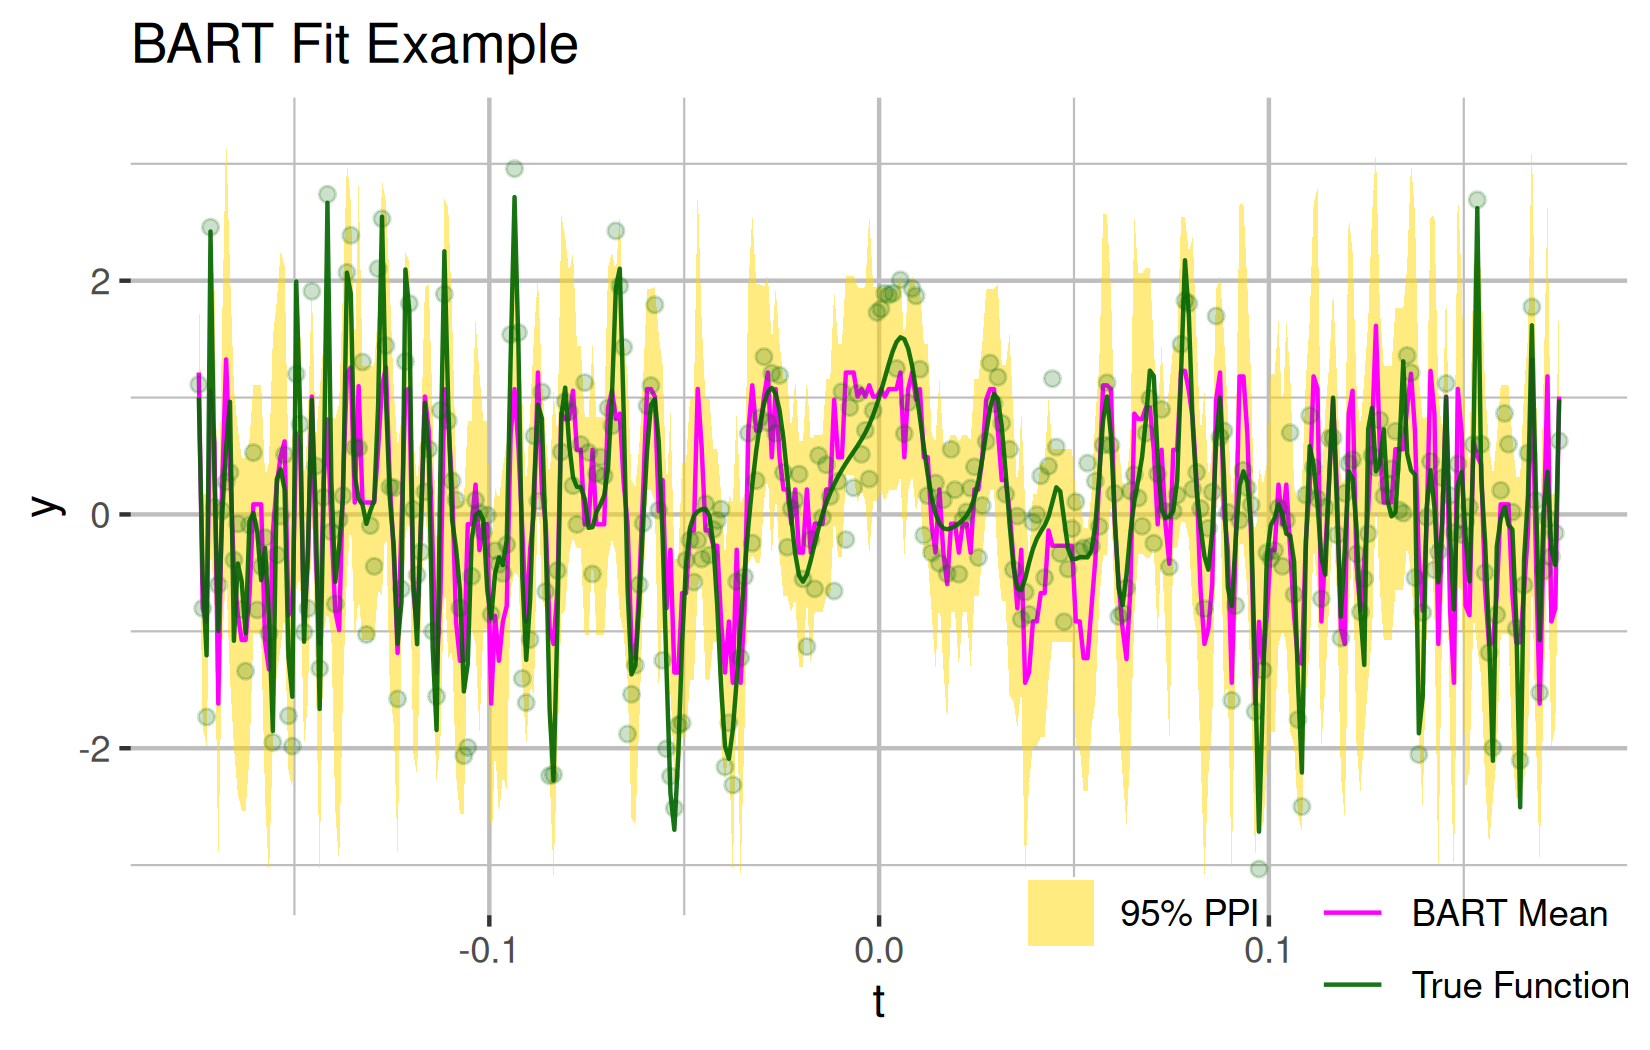
\includegraphics{main_QMD_files/figure-pdf/fig-bart-sim1-1.png}

}

\caption{\label{fig-bart-sim1}Visualization of bart}

\end{figure}%

Ensembles of trees are not used exclusively for prediction. Two
inferential tools that are commonly used with both random forests and
BART are variable importance and variable interaction measures. We
briefly describe these measures, using \cite{bartMan} bartMan R package.
Notes on variable importance and variable interaction measures are based
on the documentation. Similar measurements have been useful for
inference from random forests, but the calculations are different.

Variable importance can be measured by looking at the proportion of
decisions in which a variable is used. For BART, the structure of the
trees varies across iterations of MCMC, so we define \(c_{r,k}\) as the
number of times variable \(r\) is used as a splitting decisions within
the \(k'\)th posterior sample. \(c_k=\sum_{j=1}^Pc_{r,k}\) is thus the
total number of decisions for the \(k'\)th posterior sample. Variable
importance is then measured as
\(\text{VImp}_r=\sum_{k=1}^K\frac{c_{r,k}}{c_k}\). Thinking of the
extreme cases, with covariates that provide no information about the
response, we should simply estimate \(f\) as the mean of the observed
data. BART will make few decisions in this scenario as proposals will
provide little to no improvement to the likelihood. If we had some
variable that completely explained our response, BART may consistently
make decisions off values of said feature.

Similar to how variable importance is measured, we can assess the
potential for interactions by calculating the proportion of successive
decisions concerning two variables across posterior samples. Individual
decisions/sequences of decisions do not have much meaning on there own,
making these algorithms hard to explain. It makes sense though that if a
variable is consistently used, it must be able to explain the response
to some degree. These tools can be used to interpret a BART model, or to
help with variable selection for another model.
Figure~\ref{fig-vimp_vint} displays a matrix of variable importance and
interaction measures for data simulated under as
\(Y=X_1(X_2 + X_3+X_6)+X_2\cdot X_6+\sin(X_1)+\cos(X_2)+\log(|X_3|)+X_4^2+\lfloor X_5\rfloor+\lceil X_6\rceil+\epsilon\).
We see all interactions are found, but the plot suggests some evidence
of an interaction between \(X_3\) and \(X_6\). The coefficient of
variation is a measure used to compare one variable to another and does
not have much meaning on it's own. Like any other measure in statistics,
results must be scrutinized.

\begin{figure}[H]

\centering{

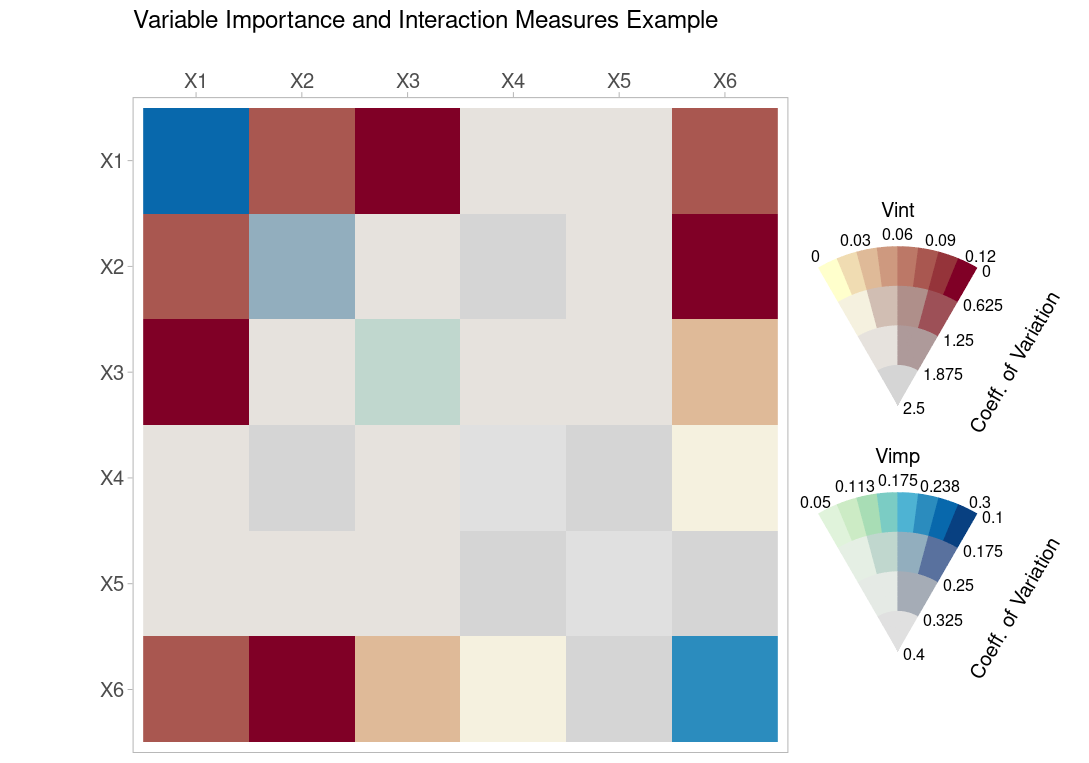
\includegraphics{figures/vimp_pres.png}

}

\caption{\label{fig-vimp_vint}Coefficient of variation matrix for
variable importance and interaction}

\end{figure}%

Before we move on to the data, we briefly discuss diagnostics for BART.
Unlike the random forest algorithm, a BART model for a continuous
response assumes normally distributed errors and constant variance. When
using a BART model, we need to assess the normality assumption, model
fit, and convergence. The bartMan R package \cite{bartMan} provides a
convenient tool for diagnostics. Figure~\ref{fig-bart_diag} shows the
diagnostics for the same model used for Figure~\ref{fig-vimp_vint}. The
Q-Q plot and Histogram both indicate normality was reasonable as
expected. We see constant variance is reasonable as well in the Fitted
vs Residuals Plot. The actual vs fitted plot shows BART fits the data
quite well as the observed and fitted values are quite close. Variable
Importance intervals shows BART correctly identified all Variables as
important as the intervals do not contain zero. The trace plot for
\(\sigma\) shows the standard deviation has converged reasonably well.
BART models have many parameters, and it is not unheard of to avoid
assessing the convergence of each tree. The thought behind this is we
don't care about any of the individual trees, so as long as our
predictions have converged the model fits reasonably well. Changing the
number of trees, along with \(\alpha\) and \(\beta\) can help with
convergence.

\begin{figure}[H]

\centering{

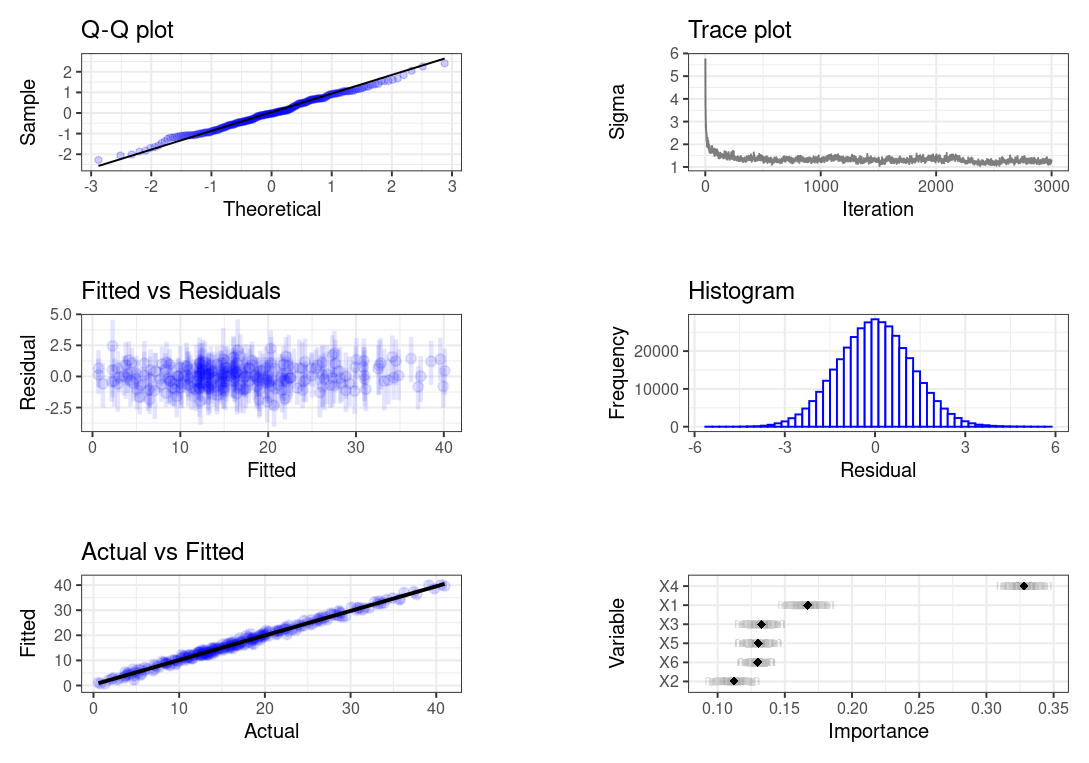
\includegraphics{figures/bart_diag.png}

}

\caption{\label{fig-bart_diag}Diagnostic plots for BART}

\end{figure}%

\section{Data}\label{sec:Data}

Before we can apply any of the models discussed to assess the importance
of land cover on flying fox feeding locations, we need to extract and
transform the data. The flying fox locations themselves form a point
pattern, which can't be modeled directly by any of the algorithms
discussed. Point patterns are a realization of a point process, defined
by a random number of observations in random locations. Modelling point
pattern data requires estimating the mean occurrence rate across an
entire surface. We're not particularly interested in the precise
locations flying foxes feed so modelling a point pattern is overkill.
Instead, we focus on the land cover characteristics of larger grid cells
to examine the potential association with feeding locations. In this
section we discuss the tools used to obtain and process our data.

\subsection{Raster Data and Google Earth
Engine}\label{raster-data-and-google-earth-engine}

Rasters are used to store data with spatial components. Each pixel has
an \((x,y)\) coordinate, and a variable of interest. We can visualize
rasters by mapping the variable to a color. Gradient scales can be used
for continuous values. For this project, we use rasters pulled via
Google Earth Engine (GEE), \cite{gee}. GEE has a large database of
satellite images and rasters of estimated attributes. Many earth engine
datasets contain images describing different attributes of the land.
These attributes are labelled bands.

An important component of spatial rasters is the coordinate reference
system (CRS). We can think about the satellite images as pictures of a
sphere. Using the position of the camera and other factors such as
distance to the earth, \((x,y,z)\) coordinates can be assigned to each
pixel. For spatial data, we need to know how far apart locations are on
the sphere. Looking at a picture of a sphere, we can't determine how far
apart points are due to the curvature. Gauss's Theorema Egregium implies
that no 2d map perfectly portrays the distance between points. We need
to choose a CRS that preserves the distance between points for our area
of interest reasonably well. The location on the earth and size of the
area determine this choice. Each raster has a pre-specified CRS that may
or may not be suitable, but rasters can always be projected into another
CRS.

Working with data from earth engine we can either select an individual
image, or an image collection. An image corresponds to a specific band
and time, while the image collection is the entire data set. When either
is selected, we have access to every time and location available. With
an image, we can clip area of interest, masking data outside this
region. With an image collection, we can filter the dataset to a
specific region and time period. After selecting a band, an individual
image can be chosen. Alternatively, we can produce an image based
calculation over the filtered time period and region. Images can then be
exported to Google Drive and can be loaded into with the R raster
package, \cite{raster}. After loading the raster, we can create a long
formatted data structure for modelling.

\subsection{Land Cover and Dynamic
World}\label{land-cover-and-dynamic-world}

One category of datasets on Google Earth Engine is land cover. Land
cover describes natural and developed features of the earth as classes.
A similar but distinct class of datasets is land use, which describes
how humans use the land. There are various methods to estimate land
cover, and many models estimate different classes. Additionally,
different datasets span various regions and time periods. The majority
of land cover datasets are annual and not quite up to date. Estimates
are produced in a multi-phase modelling process, considering many images
along with external prior information. Working with recent data from
Australia, there are fewer options, especially after excluding low
resolution datasets. In this project, we utilize data from DynamicWorld
V1 by \cite{dynamic_world}. Dynamic World is a daily high resolution
land cover dataset derived from Sentinel-2 satellites. The estimated
probability of each class in dynamic world is the output from a
convectional neural nets predictions on a single satellite image.

Within Dynamic World there are ten bands, each containing a collection
of images at a \(10\ m\) resolution. In our analysis, we use eight
relevant bands that each contain the estimated probability that a
\(100\ m^2\) region of the earth corresponds to the chosen band.
Unsurprisingly, daily high resolution data is rife with missingness. To
combat this, we compute the median land class over a selected period of
time. Missing values are ignored in the calculation by default. This
also helps slightly with the fact that Dynamic World estimates are based
on an individual day. Weather and atmospheric factors may influence
estimates so looking at the closest day may not be advisable. We don't
expect major changes to land cover in a short period of time so this is
reasonable. An individual image can then be produced based on some
function of the images. A panel of the exported rasters is displayed in
Figure~\ref{fig-dw-lc}.

\begin{figure}[H]

\centering{

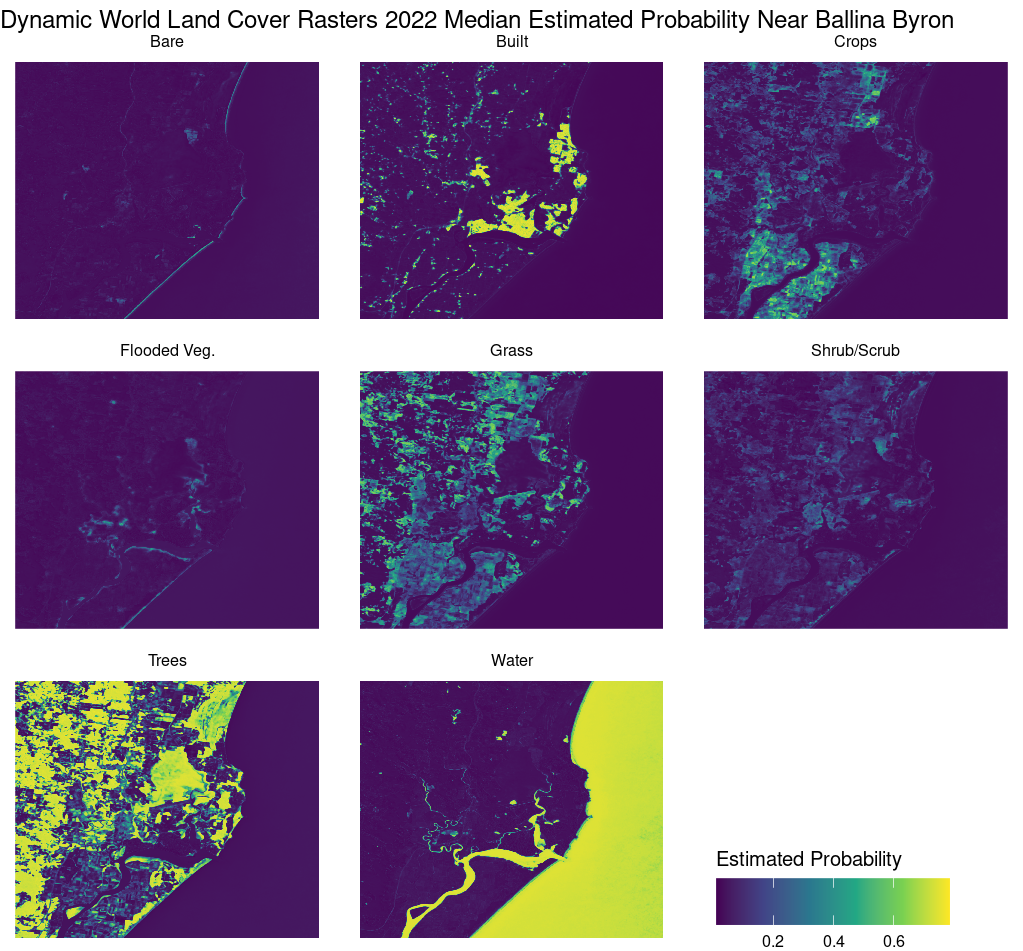
\includegraphics{figures/2022_rast.png}

}

\caption{\label{fig-dw-lc}Dynamic World Exports from Google Earth
Engine}

\end{figure}%

\subsection{Data Processing}\label{data-processing}

The radar data used in our project was extracted from an archived
PostgreSQL database with three days of observations. The radar itself is
recording data day and night, and sees many objects and organisms other
than bats. Birds and bats are essentially the same to the radar. Our
first step in processing the data was to filter observations by time and
class. Using SQL, we construct a table of flight paths for the three
sizes (classes) of bat where the last observed location is recorded
between 12:00 am and 5:00 am. The flight paths are recorded as
linestrings, a geometry representing the path through a sequence of
locations.

Using our table of linestrings, we define an area of observation for the
bats with the ST\_ConcaveHull from PostGIS. The concave hull function
takes a geometry or table of geometries, and shrink wraps a polygon
around them. There is a parameter to control the convexity, which we set
to 0.99, allowing minimal concavity. The polygon returned by
ST\_ConcaveHull along with the final observed location of bats were then
exported for additional data processing.

Any form of spatial data can be transformed into areal data by defining
a grid and aggregating observations within the cells. Before aggregating
flying fox counts, we need to define a grid. Returning to Google Earth
Engine, the previously defined boundary is imported, an enclosing
rectangle defined. The coveringGrid function is then used to define our
grid. The grid can be filtered based on our area of interest. Using the
filtered grid we, sample pixel values from dynamic world to obtain the
mean probability for each class over the grid. Resampling in earth
engine is much easier than manually averaging as we don't have to worry
about weighting averages when grid cells don't align with the cells of
rasters. Without paying additional fees, the number of cells that can be
resampled is capped at 5000. For a larger area, the grid could be
partitioned into blocks to resample in batches. At a scale of
\(289.6\ m\), our grid contains 4748 observed locations. There is slight
variation in the size of the grid, ranging from \(73,212\) to \(73,381\)
\(m^2\).

Our gridded area of interest was then imported into R along with the
three nights of radar data. Using the lengths and st\_intersect function
from the sf package \citep{sf}, we can easily obtain flying fox counts
for each grid cell. Figure~\ref{fig-proc-dat} shows our processed data
rasterized.

\begin{figure}[H]

\centering{

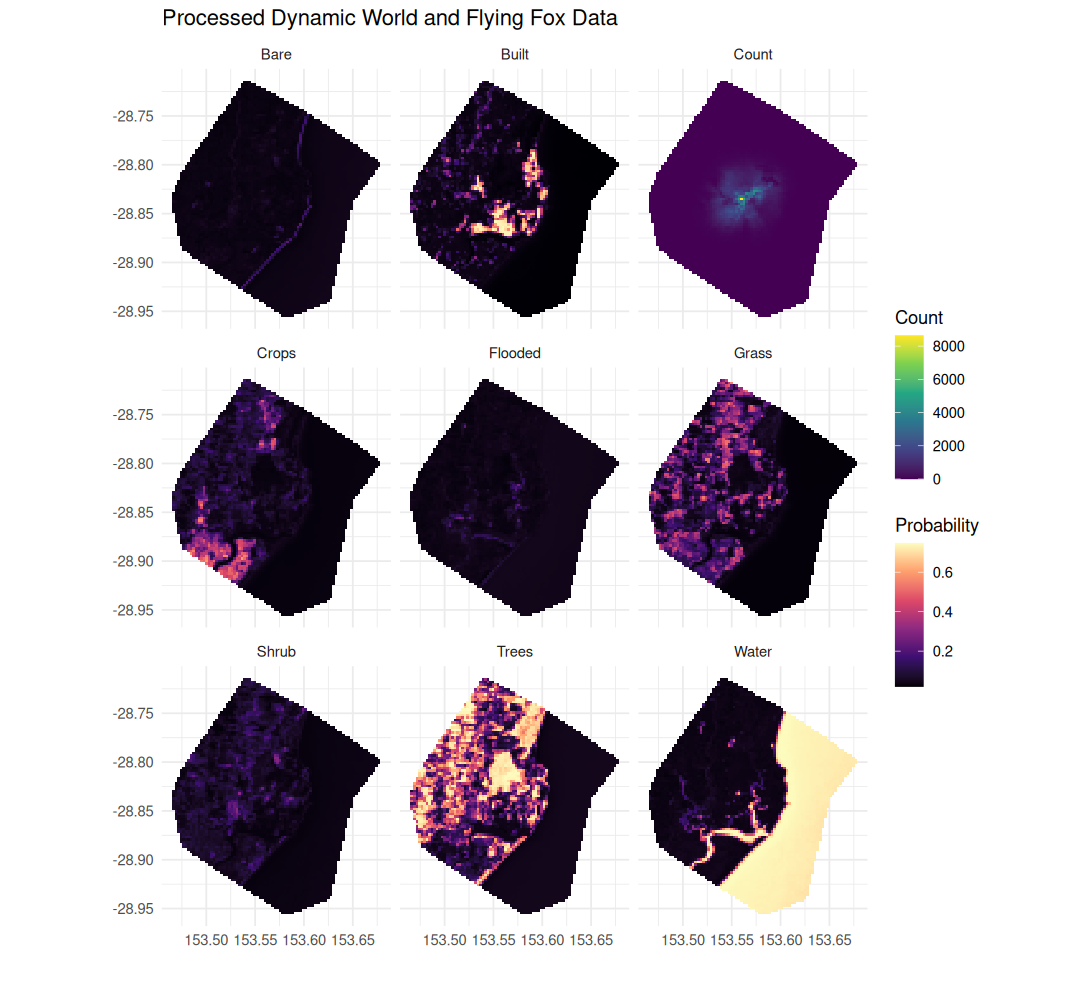
\includegraphics{figures/proc_rast.png}

}

\caption{\label{fig-proc-dat}Rasterized data for modelling}

\end{figure}%

\section{Modelling and Results}\label{modelling-and-results}

CRPS on test summary stats

\begin{longtable}[]{@{}
  >{\raggedright\arraybackslash}p{(\columnwidth - 16\tabcolsep) * \real{0.0423}}
  >{\raggedleft\arraybackslash}p{(\columnwidth - 16\tabcolsep) * \real{0.1268}}
  >{\raggedleft\arraybackslash}p{(\columnwidth - 16\tabcolsep) * \real{0.1268}}
  >{\raggedleft\arraybackslash}p{(\columnwidth - 16\tabcolsep) * \real{0.1268}}
  >{\raggedleft\arraybackslash}p{(\columnwidth - 16\tabcolsep) * \real{0.1268}}
  >{\raggedleft\arraybackslash}p{(\columnwidth - 16\tabcolsep) * \real{0.1268}}
  >{\raggedleft\arraybackslash}p{(\columnwidth - 16\tabcolsep) * \real{0.1268}}
  >{\raggedleft\arraybackslash}p{(\columnwidth - 16\tabcolsep) * \real{0.1268}}
  >{\raggedleft\arraybackslash}p{(\columnwidth - 16\tabcolsep) * \real{0.0704}}@{}}
\toprule\noalign{}
\begin{minipage}[b]{\linewidth}\raggedright
\end{minipage} & \begin{minipage}[b]{\linewidth}\raggedleft
min
\end{minipage} & \begin{minipage}[b]{\linewidth}\raggedleft
Q1
\end{minipage} & \begin{minipage}[b]{\linewidth}\raggedleft
median
\end{minipage} & \begin{minipage}[b]{\linewidth}\raggedleft
Q3
\end{minipage} & \begin{minipage}[b]{\linewidth}\raggedleft
max
\end{minipage} & \begin{minipage}[b]{\linewidth}\raggedleft
mean
\end{minipage} & \begin{minipage}[b]{\linewidth}\raggedleft
sd
\end{minipage} & \begin{minipage}[b]{\linewidth}\raggedleft
n
\end{minipage} \\
\midrule\noalign{}
\endhead
\bottomrule\noalign{}
\endlastfoot
& 1.698844 & 2.508068 & 26.02851 & 128.1026 & 4770.276 & 148.9698 &
341.4991 & 1425 \\
\end{longtable}

\begin{figure}[H]

{\centering 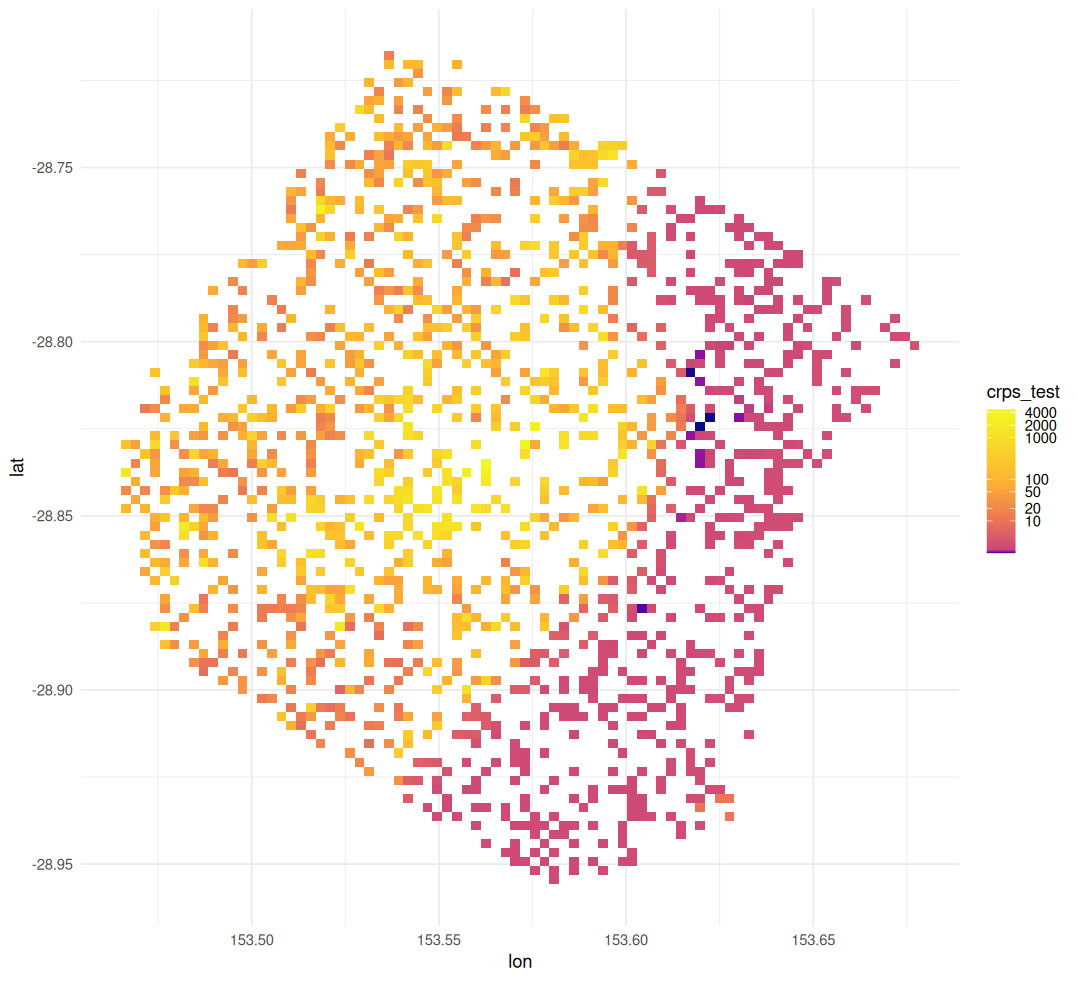
\includegraphics{figures/crps_examp.png}

}

\caption{Early results}

\end{figure}%


\renewcommand\refname{Conclusion}
  \bibliography{references.bib}



\end{document}
